\scanpage{67}

$X$ schéma projectif sur $k$,\qquad $\Gamma(X,\underline O_X)\simeq k$

$C$ son cône \unsure{projetant} affine, $a$ son sommet

$\hat C$ le cône projetant projectif

\margin{\diagram{\begin{tikzcd}[column sep=small,row sep=large]
X\arrow[r,dash,"i"]\arrow[d]&X'\arrow[r,"\pi"]\arrow[d,"f"]&X\\
a\arrow[r]&\hat C\arrow[r,dash]&{}
\end{tikzcd}}
\unsure{conditions} en II 8.7.5.}

\deleted{\diagram{\begin{tikzcd}
\operatorname{Pic}(X)\arrow[r,"\pi^*","\sim"']&\operatorname{Pic}(X')
\end{tikzcd}}}
[Car $X'$ est un fibré projectif sur $X$]

donc
\[
\operatorname{Pic}(X')\overset{\unsure{\pi^*|f^*}}{\simeq}\operatorname{Pic}(X)\times Z
\]
\deleted{[$\unsure{\underline O_{X'}(1)}$]}
\inserted{$i^*:\operatorname{Pic}(X')\mathbin{-}\operatorname{Pic}(X)$ a un noyau
$\simeq Z$, engendré par $\underline O_{X'}(1)$}

\[
\operatorname{Pic}(\hat C)\longrightarrow\operatorname{Pic}(X')
\quad\text{injectif}\quad[\text{car }f_*(\underline O_{X'})=\underline O_{\hat C}]
\]
par II 8.8.6.

\unsure{Il} s'ensuit que
\figure{\begin{tikzpicture}
\node[draw,rectangle,inner sep=8pt] (b) at (0,0)
 {$\operatorname{Pic}(\hat C)\simeq Z\overset{\sim}{\longrightarrow}
 \operatorname{Ker}[\operatorname{Pic}(X')\overset{i^*}{\mathbin{-}}\operatorname{Pic}(X)]$};
\draw (-2.9,.4) -- (-2.9,-.4);
\end{tikzpicture}}

\unsure{Soit|Sur} $C_X$ la \unsure{partie|part.} de $X'$ au-dessus de $C$,
c'est un fibré \unsure{vectoriel} de rang $1$ sur $X$.
Je dis que:
\[
\operatorname{Pic}(X)\overset{\sim}{\longrightarrow}\operatorname{Pic}(C_X)\qquad(?)
\]

\margin{faudrait supposer $X$ localement factoriel??}

Car l'hom est \deleted{\unsure{évidemment}} injectif, car son composé avec
$j^*:\operatorname{Pic}(C_X)\mathbin{-}\operatorname{Pic}(X)$,
\deleted{\unsure{si $j$ est la section nulle de $C_X$, est}}
\inserted{est} l'identité. Pour la \uline{surjectivité} on note que au-dessus
d'un ouvert convenable de $X$,

\margin{66}
